\documentclass[twoside]{book}

% Packages required by doxygen
\usepackage{fixltx2e}
\usepackage{calc}
\usepackage{doxygen}
\usepackage[export]{adjustbox} % also loads graphicx
\usepackage{graphicx}
\usepackage[utf8]{inputenc}
\usepackage{makeidx}
\usepackage{multicol}
\usepackage{multirow}
\PassOptionsToPackage{warn}{textcomp}
\usepackage{textcomp}
\usepackage[nointegrals]{wasysym}
\usepackage[table]{xcolor}

% Font selection
\usepackage[T1]{fontenc}
\usepackage[scaled=.90]{helvet}
\usepackage{courier}
\usepackage{amssymb}
\usepackage{sectsty}
\renewcommand{\familydefault}{\sfdefault}
\allsectionsfont{%
  \fontseries{bc}\selectfont%
  \color{darkgray}%
}
\renewcommand{\DoxyLabelFont}{%
  \fontseries{bc}\selectfont%
  \color{darkgray}%
}
\newcommand{\+}{\discretionary{\mbox{\scriptsize$\hookleftarrow$}}{}{}}

% Page & text layout
\usepackage{geometry}
\geometry{%
  a4paper,%
  top=2.5cm,%
  bottom=2.5cm,%
  left=2.5cm,%
  right=2.5cm%
}
\tolerance=750
\hfuzz=15pt
\hbadness=750
\setlength{\emergencystretch}{15pt}
\setlength{\parindent}{0cm}
\setlength{\parskip}{3ex plus 2ex minus 2ex}
\makeatletter
\renewcommand{\paragraph}{%
  \@startsection{paragraph}{4}{0ex}{-1.0ex}{1.0ex}{%
    \normalfont\normalsize\bfseries\SS@parafont%
  }%
}
\renewcommand{\subparagraph}{%
  \@startsection{subparagraph}{5}{0ex}{-1.0ex}{1.0ex}{%
    \normalfont\normalsize\bfseries\SS@subparafont%
  }%
}
\makeatother

% Headers & footers
\usepackage{fancyhdr}
\pagestyle{fancyplain}
\fancyhead[LE]{\fancyplain{}{\bfseries\thepage}}
\fancyhead[CE]{\fancyplain{}{}}
\fancyhead[RE]{\fancyplain{}{\bfseries\leftmark}}
\fancyhead[LO]{\fancyplain{}{\bfseries\rightmark}}
\fancyhead[CO]{\fancyplain{}{}}
\fancyhead[RO]{\fancyplain{}{\bfseries\thepage}}
\fancyfoot[LE]{\fancyplain{}{}}
\fancyfoot[CE]{\fancyplain{}{}}
\fancyfoot[RE]{\fancyplain{}{\bfseries\scriptsize Generated by Doxygen }}
\fancyfoot[LO]{\fancyplain{}{\bfseries\scriptsize Generated by Doxygen }}
\fancyfoot[CO]{\fancyplain{}{}}
\fancyfoot[RO]{\fancyplain{}{}}
\renewcommand{\footrulewidth}{0.4pt}
\renewcommand{\chaptermark}[1]{%
  \markboth{#1}{}%
}
\renewcommand{\sectionmark}[1]{%
  \markright{\thesection\ #1}%
}

% Indices & bibliography
\usepackage{natbib}
\usepackage[titles]{tocloft}
\setcounter{tocdepth}{3}
\setcounter{secnumdepth}{5}
\makeindex

% Hyperlinks (required, but should be loaded last)
\usepackage{ifpdf}
\ifpdf
  \usepackage[pdftex,pagebackref=true]{hyperref}
\else
  \usepackage[ps2pdf,pagebackref=true]{hyperref}
\fi
\hypersetup{%
  colorlinks=true,%
  linkcolor=blue,%
  citecolor=blue,%
  unicode%
}

% Custom commands
\newcommand{\clearemptydoublepage}{%
  \newpage{\pagestyle{empty}\cleardoublepage}%
}

\usepackage{caption}
\captionsetup{labelsep=space,justification=centering,font={bf},singlelinecheck=off,skip=4pt,position=top}

%===== C O N T E N T S =====

\begin{document}

% Titlepage & ToC
\hypersetup{pageanchor=false,
             bookmarksnumbered=true,
             pdfencoding=unicode
            }
\pagenumbering{roman}
\begin{titlepage}
\vspace*{7cm}
\begin{center}%
{\Large Print IP }\\
\vspace*{1cm}
{\large Generated by Doxygen 1.8.11}\\
\end{center}
\end{titlepage}
\clearemptydoublepage
\tableofcontents
\clearemptydoublepage
\pagenumbering{arabic}
\hypersetup{pageanchor=true}

%--- Begin generated contents ---
\chapter{otus\+\_\+cpp\+\_\+h4}
\label{md_README}
\hypertarget{md_README}{}
\input{md_README}
\chapter{File Index}
\section{File List}
Here is a list of all files with brief descriptions\+:\begin{DoxyCompactList}
\item\contentsline{section}{\hyperlink{print__ip_8cpp}{print\+\_\+ip.\+cpp} }{\pageref{print__ip_8cpp}}{}
\item\contentsline{section}{\hyperlink{print__ip_8h}{print\+\_\+ip.\+h} }{\pageref{print__ip_8h}}{}
\item\contentsline{section}{\hyperlink{print__ip__test_8cpp}{print\+\_\+ip\+\_\+test.\+cpp} }{\pageref{print__ip__test_8cpp}}{}
\end{DoxyCompactList}

\chapter{File Documentation}
\hypertarget{print__ip_8cpp}{}\section{print\+\_\+ip.\+cpp File Reference}
\label{print__ip_8cpp}\index{print\+\_\+ip.\+cpp@{print\+\_\+ip.\+cpp}}
{\ttfamily \#include \char`\"{}print\+\_\+ip.\+h\char`\"{}}\\*
Include dependency graph for print\+\_\+ip.\+cpp\+:
\nopagebreak
\begin{figure}[H]
\begin{center}
\leavevmode
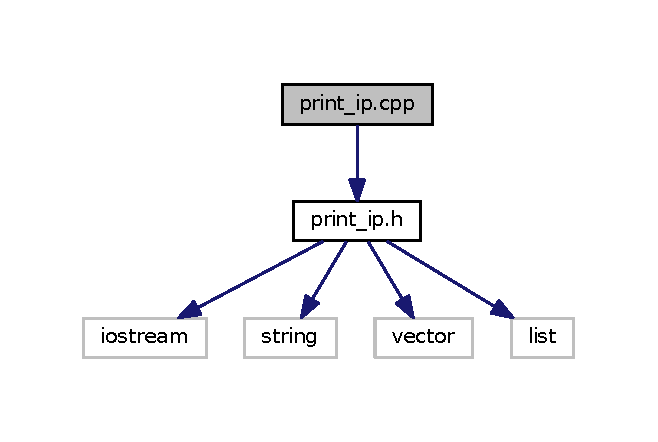
\includegraphics[width=316pt]{print__ip_8cpp__incl}
\end{center}
\end{figure}
\subsection*{Functions}
\begin{DoxyCompactItemize}
\item 
int \hyperlink{print__ip_8cpp_ae66f6b31b5ad750f1fe042a706a4e3d4}{main} ()
\end{DoxyCompactItemize}


\subsection{Function Documentation}
\index{print\+\_\+ip.\+cpp@{print\+\_\+ip.\+cpp}!main@{main}}
\index{main@{main}!print\+\_\+ip.\+cpp@{print\+\_\+ip.\+cpp}}
\subsubsection[{\texorpdfstring{main()}{main()}}]{\setlength{\rightskip}{0pt plus 5cm}int main (
\begin{DoxyParamCaption}
{}
\end{DoxyParamCaption}
)}\hypertarget{print__ip_8cpp_ae66f6b31b5ad750f1fe042a706a4e3d4}{}\label{print__ip_8cpp_ae66f6b31b5ad750f1fe042a706a4e3d4}

\hypertarget{print__ip_8h}{}\section{print\+\_\+ip.\+h File Reference}
\label{print__ip_8h}\index{print\+\_\+ip.\+h@{print\+\_\+ip.\+h}}
{\ttfamily \#include $<$iostream$>$}\\*
{\ttfamily \#include $<$string$>$}\\*
{\ttfamily \#include $<$vector$>$}\\*
{\ttfamily \#include $<$list$>$}\\*
Include dependency graph for print\+\_\+ip.\+h\+:
\nopagebreak
\begin{figure}[H]
\begin{center}
\leavevmode
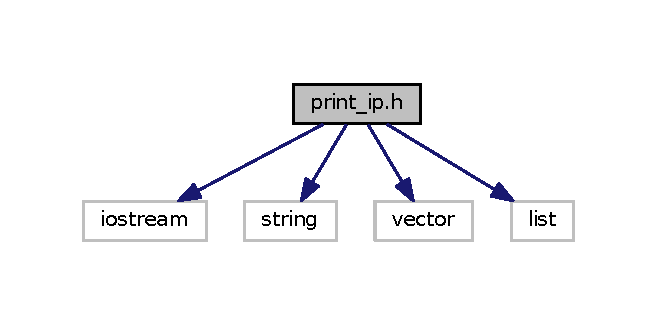
\includegraphics[width=316pt]{print__ip_8h__incl}
\end{center}
\end{figure}
This graph shows which files directly or indirectly include this file\+:
\nopagebreak
\begin{figure}[H]
\begin{center}
\leavevmode
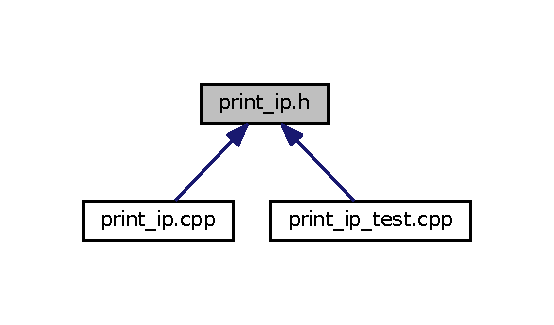
\includegraphics[width=266pt]{print__ip_8h__dep__incl}
\end{center}
\end{figure}
\subsection*{Functions}
\begin{DoxyCompactItemize}
\item 
{\footnotesize template$<$typename T $>$ }\\void \hyperlink{print__ip_8h_a3610f420073a0b75d0c002a55d706366}{print\+\_\+ip} (T param, std\+::ostream \&os)
\item 
{\footnotesize template$<$$>$ }\\void \hyperlink{print__ip_8h_a24e735d0445025c188d4f9c941b6f8cd}{print\+\_\+ip} (std\+::string param, std\+::ostream \&os)
\item 
{\footnotesize template$<$typename T $>$ }\\void \hyperlink{print__ip_8h_a0166df75eb7e4104280cc0845d5f379d}{print\+\_\+ip} (std\+::vector$<$ T $>$ param, std\+::ostream \&os)
\item 
{\footnotesize template$<$typename T $>$ }\\void \hyperlink{print__ip_8h_a86024a4cbaa0cdfdaaa8a9fed1636480}{print\+\_\+ip} (std\+::list$<$ T $>$ param, std\+::ostream \&os)
\end{DoxyCompactItemize}
\subsection*{Variables}
\begin{DoxyCompactItemize}
\item 
const int \hyperlink{print__ip_8h_a45e94606e7bad962ffc17961ee1293c2}{c\+\_\+byte\+Size} = 8
\end{DoxyCompactItemize}


\subsection{Function Documentation}
\index{print\+\_\+ip.\+h@{print\+\_\+ip.\+h}!print\+\_\+ip@{print\+\_\+ip}}
\index{print\+\_\+ip@{print\+\_\+ip}!print\+\_\+ip.\+h@{print\+\_\+ip.\+h}}
\subsubsection[{\texorpdfstring{print\+\_\+ip(\+T param, std\+::ostream \&os)}{print_ip(T param, std::ostream &os)}}]{\setlength{\rightskip}{0pt plus 5cm}template$<$typename T $>$ void print\+\_\+ip (
\begin{DoxyParamCaption}
\item[{T}]{param, }
\item[{std\+::ostream \&}]{os}
\end{DoxyParamCaption}
)}\hypertarget{print__ip_8h_a3610f420073a0b75d0c002a55d706366}{}\label{print__ip_8h_a3610f420073a0b75d0c002a55d706366}
\index{print\+\_\+ip.\+h@{print\+\_\+ip.\+h}!print\+\_\+ip@{print\+\_\+ip}}
\index{print\+\_\+ip@{print\+\_\+ip}!print\+\_\+ip.\+h@{print\+\_\+ip.\+h}}
\subsubsection[{\texorpdfstring{print\+\_\+ip(std\+::string param, std\+::ostream \&os)}{print_ip(std::string param, std::ostream &os)}}]{\setlength{\rightskip}{0pt plus 5cm}template$<$$>$ void print\+\_\+ip (
\begin{DoxyParamCaption}
\item[{std\+::string}]{param, }
\item[{std\+::ostream \&}]{os}
\end{DoxyParamCaption}
)}\hypertarget{print__ip_8h_a24e735d0445025c188d4f9c941b6f8cd}{}\label{print__ip_8h_a24e735d0445025c188d4f9c941b6f8cd}
\index{print\+\_\+ip.\+h@{print\+\_\+ip.\+h}!print\+\_\+ip@{print\+\_\+ip}}
\index{print\+\_\+ip@{print\+\_\+ip}!print\+\_\+ip.\+h@{print\+\_\+ip.\+h}}
\subsubsection[{\texorpdfstring{print\+\_\+ip(std\+::vector$<$ T $>$ param, std\+::ostream \&os)}{print_ip(std::vector< T > param, std::ostream &os)}}]{\setlength{\rightskip}{0pt plus 5cm}template$<$typename T $>$ void print\+\_\+ip (
\begin{DoxyParamCaption}
\item[{std\+::vector$<$ T $>$}]{param, }
\item[{std\+::ostream \&}]{os}
\end{DoxyParamCaption}
)}\hypertarget{print__ip_8h_a0166df75eb7e4104280cc0845d5f379d}{}\label{print__ip_8h_a0166df75eb7e4104280cc0845d5f379d}
\index{print\+\_\+ip.\+h@{print\+\_\+ip.\+h}!print\+\_\+ip@{print\+\_\+ip}}
\index{print\+\_\+ip@{print\+\_\+ip}!print\+\_\+ip.\+h@{print\+\_\+ip.\+h}}
\subsubsection[{\texorpdfstring{print\+\_\+ip(std\+::list$<$ T $>$ param, std\+::ostream \&os)}{print_ip(std::list< T > param, std::ostream &os)}}]{\setlength{\rightskip}{0pt plus 5cm}template$<$typename T $>$ void print\+\_\+ip (
\begin{DoxyParamCaption}
\item[{std\+::list$<$ T $>$}]{param, }
\item[{std\+::ostream \&}]{os}
\end{DoxyParamCaption}
)}\hypertarget{print__ip_8h_a86024a4cbaa0cdfdaaa8a9fed1636480}{}\label{print__ip_8h_a86024a4cbaa0cdfdaaa8a9fed1636480}


\subsection{Variable Documentation}
\index{print\+\_\+ip.\+h@{print\+\_\+ip.\+h}!c\+\_\+byte\+Size@{c\+\_\+byte\+Size}}
\index{c\+\_\+byte\+Size@{c\+\_\+byte\+Size}!print\+\_\+ip.\+h@{print\+\_\+ip.\+h}}
\subsubsection[{\texorpdfstring{c\+\_\+byte\+Size}{c_byteSize}}]{\setlength{\rightskip}{0pt plus 5cm}const int c\+\_\+byte\+Size = 8}\hypertarget{print__ip_8h_a45e94606e7bad962ffc17961ee1293c2}{}\label{print__ip_8h_a45e94606e7bad962ffc17961ee1293c2}

\hypertarget{print__ip__test_8cpp}{}\section{print\+\_\+ip\+\_\+test.\+cpp File Reference}
\label{print__ip__test_8cpp}\index{print\+\_\+ip\+\_\+test.\+cpp@{print\+\_\+ip\+\_\+test.\+cpp}}
{\ttfamily \#include $<$gtest/gtest.\+h$>$}\\*
{\ttfamily \#include $<$sstream$>$}\\*
{\ttfamily \#include \char`\"{}print\+\_\+ip.\+h\char`\"{}}\\*
Include dependency graph for print\+\_\+ip\+\_\+test.\+cpp\+:
\nopagebreak
\begin{figure}[H]
\begin{center}
\leavevmode
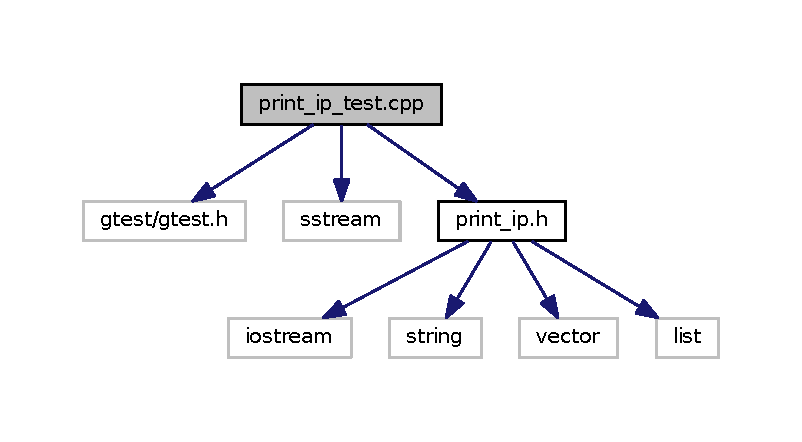
\includegraphics[width=350pt]{print__ip__test_8cpp__incl}
\end{center}
\end{figure}
\subsection*{Functions}
\begin{DoxyCompactItemize}
\item 
\hyperlink{print__ip__test_8cpp_a7df4076bbc0a749a1c32a00f195ab2ed}{T\+E\+ST} (\hyperlink{print__ip_8h_a86024a4cbaa0cdfdaaa8a9fed1636480}{print\+\_\+ip}, print\+\_\+ip\+\_\+test\+\_\+char)
\item 
\hyperlink{print__ip__test_8cpp_a16a7bdc6c0b356b0f90484af7e1af4f0}{T\+E\+ST} (\hyperlink{print__ip_8h_a86024a4cbaa0cdfdaaa8a9fed1636480}{print\+\_\+ip}, print\+\_\+ip\+\_\+test\+\_\+short)
\item 
\hyperlink{print__ip__test_8cpp_a765a036d9e84dc096599cc91216c8d89}{T\+E\+ST} (\hyperlink{print__ip_8h_a86024a4cbaa0cdfdaaa8a9fed1636480}{print\+\_\+ip}, print\+\_\+ip\+\_\+test\+\_\+int)
\item 
\hyperlink{print__ip__test_8cpp_adc958caa282dee15f1b15143df9840e6}{T\+E\+ST} (\hyperlink{print__ip_8h_a86024a4cbaa0cdfdaaa8a9fed1636480}{print\+\_\+ip}, print\+\_\+ip\+\_\+test\+\_\+long)
\item 
\hyperlink{print__ip__test_8cpp_ab573d6de148ae2b0835a7345a19c427c}{T\+E\+ST} (\hyperlink{print__ip_8h_a86024a4cbaa0cdfdaaa8a9fed1636480}{print\+\_\+ip}, print\+\_\+ip\+\_\+test\+\_\+string)
\item 
\hyperlink{print__ip__test_8cpp_ae7bdc526a076d36d168ec70aa20fbade}{T\+E\+ST} (\hyperlink{print__ip_8h_a86024a4cbaa0cdfdaaa8a9fed1636480}{print\+\_\+ip}, print\+\_\+ip\+\_\+test\+\_\+vector)
\item 
\hyperlink{print__ip__test_8cpp_aaab8b7cb7eff5af9e0abd306c944c53f}{T\+E\+ST} (\hyperlink{print__ip_8h_a86024a4cbaa0cdfdaaa8a9fed1636480}{print\+\_\+ip}, print\+\_\+ip\+\_\+test\+\_\+list)
\item 
int \hyperlink{print__ip__test_8cpp_a0ddf1224851353fc92bfbff6f499fa97}{main} (int argc, char $\ast$argv\mbox{[}$\,$\mbox{]})
\end{DoxyCompactItemize}


\subsection{Function Documentation}
\index{print\+\_\+ip\+\_\+test.\+cpp@{print\+\_\+ip\+\_\+test.\+cpp}!main@{main}}
\index{main@{main}!print\+\_\+ip\+\_\+test.\+cpp@{print\+\_\+ip\+\_\+test.\+cpp}}
\subsubsection[{\texorpdfstring{main(int argc, char $\ast$argv[])}{main(int argc, char *argv[])}}]{\setlength{\rightskip}{0pt plus 5cm}int main (
\begin{DoxyParamCaption}
\item[{int}]{argc, }
\item[{char $\ast$}]{argv\mbox{[}$\,$\mbox{]}}
\end{DoxyParamCaption}
)}\hypertarget{print__ip__test_8cpp_a0ddf1224851353fc92bfbff6f499fa97}{}\label{print__ip__test_8cpp_a0ddf1224851353fc92bfbff6f499fa97}
\index{print\+\_\+ip\+\_\+test.\+cpp@{print\+\_\+ip\+\_\+test.\+cpp}!T\+E\+ST@{T\+E\+ST}}
\index{T\+E\+ST@{T\+E\+ST}!print\+\_\+ip\+\_\+test.\+cpp@{print\+\_\+ip\+\_\+test.\+cpp}}
\subsubsection[{\texorpdfstring{T\+E\+S\+T(print\+\_\+ip, print\+\_\+ip\+\_\+test\+\_\+char)}{TEST(print_ip, print_ip_test_char)}}]{\setlength{\rightskip}{0pt plus 5cm}T\+E\+ST (
\begin{DoxyParamCaption}
\item[{{\bf print\+\_\+ip}}]{, }
\item[{print\+\_\+ip\+\_\+test\+\_\+char}]{}
\end{DoxyParamCaption}
)}\hypertarget{print__ip__test_8cpp_a7df4076bbc0a749a1c32a00f195ab2ed}{}\label{print__ip__test_8cpp_a7df4076bbc0a749a1c32a00f195ab2ed}
\index{print\+\_\+ip\+\_\+test.\+cpp@{print\+\_\+ip\+\_\+test.\+cpp}!T\+E\+ST@{T\+E\+ST}}
\index{T\+E\+ST@{T\+E\+ST}!print\+\_\+ip\+\_\+test.\+cpp@{print\+\_\+ip\+\_\+test.\+cpp}}
\subsubsection[{\texorpdfstring{T\+E\+S\+T(print\+\_\+ip, print\+\_\+ip\+\_\+test\+\_\+short)}{TEST(print_ip, print_ip_test_short)}}]{\setlength{\rightskip}{0pt plus 5cm}T\+E\+ST (
\begin{DoxyParamCaption}
\item[{{\bf print\+\_\+ip}}]{, }
\item[{print\+\_\+ip\+\_\+test\+\_\+short}]{}
\end{DoxyParamCaption}
)}\hypertarget{print__ip__test_8cpp_a16a7bdc6c0b356b0f90484af7e1af4f0}{}\label{print__ip__test_8cpp_a16a7bdc6c0b356b0f90484af7e1af4f0}
\index{print\+\_\+ip\+\_\+test.\+cpp@{print\+\_\+ip\+\_\+test.\+cpp}!T\+E\+ST@{T\+E\+ST}}
\index{T\+E\+ST@{T\+E\+ST}!print\+\_\+ip\+\_\+test.\+cpp@{print\+\_\+ip\+\_\+test.\+cpp}}
\subsubsection[{\texorpdfstring{T\+E\+S\+T(print\+\_\+ip, print\+\_\+ip\+\_\+test\+\_\+int)}{TEST(print_ip, print_ip_test_int)}}]{\setlength{\rightskip}{0pt plus 5cm}T\+E\+ST (
\begin{DoxyParamCaption}
\item[{{\bf print\+\_\+ip}}]{, }
\item[{print\+\_\+ip\+\_\+test\+\_\+int}]{}
\end{DoxyParamCaption}
)}\hypertarget{print__ip__test_8cpp_a765a036d9e84dc096599cc91216c8d89}{}\label{print__ip__test_8cpp_a765a036d9e84dc096599cc91216c8d89}
\index{print\+\_\+ip\+\_\+test.\+cpp@{print\+\_\+ip\+\_\+test.\+cpp}!T\+E\+ST@{T\+E\+ST}}
\index{T\+E\+ST@{T\+E\+ST}!print\+\_\+ip\+\_\+test.\+cpp@{print\+\_\+ip\+\_\+test.\+cpp}}
\subsubsection[{\texorpdfstring{T\+E\+S\+T(print\+\_\+ip, print\+\_\+ip\+\_\+test\+\_\+long)}{TEST(print_ip, print_ip_test_long)}}]{\setlength{\rightskip}{0pt plus 5cm}T\+E\+ST (
\begin{DoxyParamCaption}
\item[{{\bf print\+\_\+ip}}]{, }
\item[{print\+\_\+ip\+\_\+test\+\_\+long}]{}
\end{DoxyParamCaption}
)}\hypertarget{print__ip__test_8cpp_adc958caa282dee15f1b15143df9840e6}{}\label{print__ip__test_8cpp_adc958caa282dee15f1b15143df9840e6}
\index{print\+\_\+ip\+\_\+test.\+cpp@{print\+\_\+ip\+\_\+test.\+cpp}!T\+E\+ST@{T\+E\+ST}}
\index{T\+E\+ST@{T\+E\+ST}!print\+\_\+ip\+\_\+test.\+cpp@{print\+\_\+ip\+\_\+test.\+cpp}}
\subsubsection[{\texorpdfstring{T\+E\+S\+T(print\+\_\+ip, print\+\_\+ip\+\_\+test\+\_\+string)}{TEST(print_ip, print_ip_test_string)}}]{\setlength{\rightskip}{0pt plus 5cm}T\+E\+ST (
\begin{DoxyParamCaption}
\item[{{\bf print\+\_\+ip}}]{, }
\item[{print\+\_\+ip\+\_\+test\+\_\+string}]{}
\end{DoxyParamCaption}
)}\hypertarget{print__ip__test_8cpp_ab573d6de148ae2b0835a7345a19c427c}{}\label{print__ip__test_8cpp_ab573d6de148ae2b0835a7345a19c427c}
\index{print\+\_\+ip\+\_\+test.\+cpp@{print\+\_\+ip\+\_\+test.\+cpp}!T\+E\+ST@{T\+E\+ST}}
\index{T\+E\+ST@{T\+E\+ST}!print\+\_\+ip\+\_\+test.\+cpp@{print\+\_\+ip\+\_\+test.\+cpp}}
\subsubsection[{\texorpdfstring{T\+E\+S\+T(print\+\_\+ip, print\+\_\+ip\+\_\+test\+\_\+vector)}{TEST(print_ip, print_ip_test_vector)}}]{\setlength{\rightskip}{0pt plus 5cm}T\+E\+ST (
\begin{DoxyParamCaption}
\item[{{\bf print\+\_\+ip}}]{, }
\item[{print\+\_\+ip\+\_\+test\+\_\+vector}]{}
\end{DoxyParamCaption}
)}\hypertarget{print__ip__test_8cpp_ae7bdc526a076d36d168ec70aa20fbade}{}\label{print__ip__test_8cpp_ae7bdc526a076d36d168ec70aa20fbade}
\index{print\+\_\+ip\+\_\+test.\+cpp@{print\+\_\+ip\+\_\+test.\+cpp}!T\+E\+ST@{T\+E\+ST}}
\index{T\+E\+ST@{T\+E\+ST}!print\+\_\+ip\+\_\+test.\+cpp@{print\+\_\+ip\+\_\+test.\+cpp}}
\subsubsection[{\texorpdfstring{T\+E\+S\+T(print\+\_\+ip, print\+\_\+ip\+\_\+test\+\_\+list)}{TEST(print_ip, print_ip_test_list)}}]{\setlength{\rightskip}{0pt plus 5cm}T\+E\+ST (
\begin{DoxyParamCaption}
\item[{{\bf print\+\_\+ip}}]{, }
\item[{print\+\_\+ip\+\_\+test\+\_\+list}]{}
\end{DoxyParamCaption}
)}\hypertarget{print__ip__test_8cpp_aaab8b7cb7eff5af9e0abd306c944c53f}{}\label{print__ip__test_8cpp_aaab8b7cb7eff5af9e0abd306c944c53f}

\hypertarget{_r_e_a_d_m_e_8md}{}\section{R\+E\+A\+D\+M\+E.\+md File Reference}
\label{_r_e_a_d_m_e_8md}\index{R\+E\+A\+D\+M\+E.\+md@{R\+E\+A\+D\+M\+E.\+md}}

%--- End generated contents ---

% Index
\backmatter
\newpage
\phantomsection
\clearemptydoublepage
\addcontentsline{toc}{chapter}{Index}
\printindex

\end{document}
